\documentclass[11pt,a4paper]{article}

\usepackage{tpacdc}
\usepackage{hyperref}
\usepackage[normalem]{ ulem }
\usepackage{soul}
\usepackage{siunitx}
\usepackage{graphicx}
\usepackage{blindtext} % USE FOR LOREM IPSUM

% Custom colors
\usepackage{color}
\definecolor{deepblue}{rgb}{0,0,0.5}
\definecolor{deepred}{rgb}{0.6,0,0}
\definecolor{deepgreen}{rgb}{0,0.5,0}
\definecolor{gray}{rgb}{0.5,0.5,0.5}

\usepackage{listings}
\lstset{
  language=Python,
  basicstyle=\ttfamily\small,
  frame=single,
  numbers=left,
  keywordstyle=\color{deepblue},
  emphstyle=\color{deepred},
  stringstyle=\color{deepgreen},
  commentstyle=\color{gray},
  showstringspaces=false,
  keepspaces=true,
  inputencoding=utf8,
  extendedchars=true,
  literate={é}{{\'e}}1
           {°}{{\textdegree}}1,
  escapeinside={\%*}{*)}
}

\textheight 24cm
\textwidth 16cm
\oddsidemargin 0cm
\topmargin -0.5cm

\begin{document}
\[\enteteTPCS{1.0}{Immersion}{2018}{Le Jeu de la Vie}{Une fable de Jean-Michel Jéquonfe}

% Consignes de rendu
\section{Introduction}
L'objectif de cet atelier est de vous montrer quelques bases de
programmation dans un langage très simple pour débuter~: le Python.

Vous êtes encadrés par plusieurs étudiants et enseignants de l'EPITA. N'hésitez
pas à nous poser des questions !

Le but de cet atelier est de vous faire programmer ce qu'on appelle un game of life à l'aide
\emph{Python}\footnote{\url{http://python.org/}} et de son module
\emph{tkinter}\footnote{\url{https://docs.python.org/3/library/tkinter.html}},
un ensemble d'outils destiné à un affichage graphique plus poussé que \emph{turtle}.  
Vous trouverez en annexe un aperçu du rendu final.

\section{L'environnement de développement}
\subsection{Généralités}

Dans un premier temps, regardons l'environnement qui sera utilisé pour réaliser
cet atelier. Un environnement de développement est généralement composé de trois
outils~:

\begin{itemize}
    \item un éditeur~: l'espace éditable où vous taperez votre code~;
    \item un compilateur~: un logiciel qui traduira le code que vous aurez
        écrit afin qu'il soit compréhensible par l'ordinateur. Pour certains
        langages, ce compilateur est remplacé par un interpréteur (la différence
        n'a pas d'importance ici)~;
    \item un debugger~: un outil nous permettant d'analyser notre programme afin
        de corriger les erreurs qui s'y sont glissées.
\end{itemize}

Vous avez de la chance, il existe des logiciel qui combinent éditeur et
compilateur / interpréteur. On les appelle IDE (Integrated Development
Environnement - Environnement de développement intégré).

\subsection{Votre environnement}

Pour cet atelier, nous vous proposons d'utiliser un IDE pour faciliter
les différents tests. Celui-ci est décomposer en deux parties, une console
et un éditeur de texte. La console permet d'exécuter facilement des instructions,
et l'éditeur permet de faire des programmes autrement dit des ensembles d'instructions.

\begin{itemize}
    \item Rappelons maintenant certaines lignes de code utile à la compréhension du TP:
        \begin{itemize}
            \item \lstinline{#l is a list} est un commentaire, il sera
                ignoré par l'interpréteur, comme toutes les lignes commençant
                par \lstinline{#}.  Les commentaires permettent d'aider les
                humains qui lisent le code du programme (un collègue, un ami, ou
                vous-même plusieurs jours après)~;
            \item \lstinline{l.append(1)}~: premier exemple de ligne de code
                que vous allez utiliser pendant l'atelier, cette ligne ajoute
                Le chiffre 1 à la liste l. Toute instruction terminant par \lstinline{()}
                est considéré comme une fonction par python. Ici, append() est une fonction
                appartenant à l. Celle-ci étant une liste, dans autres mots, append() est 
                une fonction appartenant à l'objet Liste nommé ici l.
        \end{itemize}
\end{itemize}

Si vous essayez d'exécuter la ligne ci-dessus (en allant sur Run>Run Module ou via la console),
vous remarquerez que cela ne marchera uniquement si vous définissez l comme étant une liste.
C'est pour cette raison que nous aborderons les listes en premier étant essentiels à la
réalisation d'un game of life.

\section{Introductions aux listes pythoniques}

Les listes sont, comme leur nom l'indique, des objets qui contiennent un à plusieurs objets.
Grâce à celles-ci on peut facilement accéder, trier et modifier les données qu'elle contient.

\subsection{Quelques exemples de listes pour débuter}
Ci-dessous, la liste "Chiffres" contient les chiffres de 0 à 9.

\begin{lstlisting}
>>> Chiffres = [0,1,2,3,4,5,6,7,8,9]
\end{lstlisting}

Ou encore la liste "void" contenant rien du tout:

\begin{lstlisting}
>>> void = []
\end{lstlisting}

\subsection{Opération sur les listes}
Pour introduire cette partie, nous allons modifier la liste Chiffres récemment créé pour introduire les manipulations 
de bases sur les listes pythoniques. Il y a deux manières de procéder, 
premièrement en ajoutant une valeur à la liste ou en modifiant une valeur existante sur la liste.

Notons que la fonction print() affiche son paramètre (=ce qui est contenu dans les parenthèses).
\begin{lstlisting}
>>> Chiffres.append(89) #Ajoute le chiffre 89 à la fin de la liste
>>> print(Chiffres) #Affiche la liste Chiffres
[0,1,2,3,4,5,6,7,8,9,89]
\end{lstlisting}

La forme suivante : liste[index] possède un index qui commence à 0 jusqu'a la longueur de la liste - 1
En outre : liste[0] s'adresse au premier élément de la liste, liste[4] s'adresse au cinquième.

\begin{lstlisting}
>>> Chiffres[10] = 42 #Modifie la valeur en position 10 par 42
>>> print(Chiffres)
[0,1,2,3,4,5,6,7,8,9,42]
\end{lstlisting}

Notez que liste[index] renvoi l'élément en position index :
\begin{lstlisting} 
>>> Chiffres[0]
0    
\end{lstlisting}

On va maintenant supprimer un élément de la liste, il existe deux manières de procéder.

\begin{lstlisting} 
#Way 1
del Chiffres[10] #supr
>>> print(Chiffres)
[0,1,2,3,4,5,6,7,8,9]

#Way 2
Chiffres.pop(0)
>>> print(Chiffres)
[1,2,3,4,5,6,7,8,9]
\end{lstlisting}

{\fontencoding{U}\fontfamily{futs}\selectfont\char 66\relax} Si l'on adresse un index inexistant lors de l'une de ces fonctions ci-dessus on obtient une erreur comme ci-dessous

\begin{lstlisting} 
>>> Chiffres[12]
[...]
IndexError: list index out of range
\end{lstlisting}


\subsection{Petit rappel : Les fonctions/procédures}

Souvent vous vous retrouverez en informatique à faire répéter plusieurs fois
la même opération à l'ordinateur, c'est pour éviter de se répéter dans le code
que nous utilisons ce que nous appelons les fonctions ou encore procédure. De cette manière
Vous pouvez répéter des opérations à l'ordinateur sans vous répéter dans le code, simplement
En appelant la fonction.

Le schéma général de déclaration de procédure est le suivant~:

\begin{lstlisting}
def nom_de_ma_super_procedure():    # on nomme la procedure
    instruction 1                   # tabulation obligatoire
    instruction 2
\end{lstlisting}

Prenez garde aux espaces avant chaque instruction~: cela permet au
compilateur/interpréteur de savoir que les instructions appartiennent
bien à la fonction\footnote{Certains langages ont une approche différente~: le
C, C++, Java, et C\# par exemple utilisent des accolades pour délimiter le corps
des fonctions. Les langages tels que Python ou encore le Haskell délimitent les
corps de fonctions par rapport à l'indentation, ce qui rend le code
\emph{naturellement} lisible.}.

Une fois définie, vous appelez votre procédure tout simplement comme
suit~:

\begin{lstlisting}
nom_de_ma_super_procedure()
\end{lstlisting}

\emph{Appeler} une procédure revient à exécuter le code qu'elle contient.

Voici quelques procédures que vous pouvez tester pour mieux comprendre :


\begin{lstlisting}
def somme_liste(liste):
  Total = 0
  for elem in liste:
    Total += elem
  return Total
\end{lstlisting}

\begin{lstlisting}
def Multiply(liste):
  Total = 0
  for i in range(len(liste)):
    Total *= liste[i]
  return Total  
\end{lstlisting}

\subsection{Créez vos propres fonctions~!}

Il est maintenant temps de créer vos propres fonctions. Voici
Quelques exercices pour compléter l'introduction aux listes. 

Exercice 1 : Boucler une liste


Créer la fonction AfficherListe(liste) qui affiche le contenu d'une liste élément par élément
Rappel : la boucle for pythonique est syntaxé de la manière suivante : 
for variable in itérable: ; plus simplement : for variable in range(nombres d'itérations max):
(range(n) génère un itérable tel une liste de 0 à n exclus, on peut également préciser la valeur de départ via range(1,3) -> [1,2])

Output Exemple:
\begin{lstlisting}
>>> liste = [1,6,4,9]
>>> AfficherListe(liste)
1
6
4
9
>>> 
\end{lstlisting}




Exercice 2 : Doubles listes (Matrices)


Créer la fonction InitBoard(largeur,hauteur,element) qui crée la Matrice de (largeur x hauteur) contenant unique element
On peut également représenter le problème comme un tableau en 2 dimension où une ligne équivaut à une liste contenant les elements
et le tableau une liste qui englobe le tout. Ainsi une élément sur une ligne se situe dans une ligne qui est englobé par le tableau.



Output Exemple:
\begin{lstlisting}
>>> InitBoard(4,3,0)
[[0, 0, 0, 0], [0, 0, 0, 0], [0, 0, 0, 0]]
\end{lstlisting}



Exercice 3 : Application avancée

Utiliser la fonction de l'exercice précédent pour générer une matrice 5x5 rempli de 0 et à l'aide du module Random,
Créer la fonction Malea(matrice,itérations,largeur,hauteur) qui modifie la matrice généré en remplaçant 
une coordonnée (x,y) aléatoire de la matrice en 1 au lieu de 0 et répète cette action itérations fois.

Rappel : Module random
Pour utiliser le module random, importez le en début de programme via : import random
Pour générer un nombre aléatoire entier entre a et b : random.randint(a,b)

Output Exemple:
\begin{lstlisting}
>>> matrice = InitBoard(4,3,0)
>>> matrice
[[0, 0, 0, 0], [0, 0, 0, 0], [0, 0, 0, 0]]
>>> Malea(matrice,7,4,3)
>>> matrice
[[1, 1, 1, 0], [1, 0, 0, 1], [0, 1, 1, 0]]
\end{lstlisting}

\section{Le Jeu : Game of Life}

Nous allons considérer notre matrice comme un tableau en 2 dimension où sur chaque élément se trouve un entier entre 0 et 1 
équivalent à l'état d'une cellule 0 <-> Morte ; 1 <=> Vivante

Ces cellules suivent des règles particulières qui détermine leur évolution génération après génération.
Ces règles sont déterminé en fonction de l'état des 8 cellules voisines de la façon suivante :
\begin{itemize}	
	\item Une cellule morte possédant exactement trois voisins vivantes devient vivante (elle naît)
	
	\item Une cellule vivante possédant deux ou trois voisins vivantes le reste sinon elle meurt (elle disparaît)
\end{itemize}

\subsection{Fonctions utiles}
Exercice 4 : Règle
Créer la fonction rule(cell,voisin) qui à partir de l'état d'une cellule et du nombre de voisins vivants retourne l'état
de la cellule à la prochaine génération lors de l'application des règle sur la cellule.
\begin{lstlisting}
>>> rule(0,3)
1
>>> rule(1,2)
1
>>> rule(1,4)
0
\end{lstlisting}

Exercice 5:
Créer la fonction count(cellx,celly,tableau) qui retourne le nombre de cellule vivante autour d'une cellule en (x,y)
sur notre tableau

\begin{lstlisting}
>>> count(1,2,tableau)
3
>>> tableau
[[0, 0, 0, 1], [0, 1, 1, 1], [1, 1, 0, 0]]
\end{lstlisting}

Exercice 6:
Créer la fonction nextgen(tableau,largeur,hauteur) qui applique rule sur tous les cellules du tableau.

Note : Les paramètres largeur et hauteur sont optionnel; il est possible de réaliser l'algorithme sans.

\begin{lstlisting}
>>> liste
[0, 0, 0, 1], [0, 1, 1, 1], [1, 1, 0, 0]]
>>> nexgen(liste,4,3)
>>> liste
[[0, 0, 1, 1], [1, 0, 0, 0], [1, 0, 0, 1]]
\end{lstlisting}

\subsection{L'interface graphique : tkinter}

Ceci est un module permettant à python de profiter d'outils graphique tels que des fenêtres et des zones de "dessin" appelés canvas.
Comme tout module, pour l'utiliser il est nécessaire de l'importer via la ligne 1. 
La ligne 2 sers à initialiser la fenêtre graphique.
Cette variable (ligne 2) va servir de référence à notre fenêtre il est donc important d'utiliser quelque chose de court 
et compréhensible tel que fen, tk etc...
La dernière ligne est à toujours mettre en fin de programme, son but est définir une boucle continue sur la fenêtre.
Cela permet de gérer plus que l'affichage tel que les cliques de la souris; les touches du claviers voir répéter une fonction tous les x temps etc...

\begin{lstlisting}
from tkinter import *
fen = Tk()
#...
#...
fen.mainloop()
\end{lstlisting}

Pour dessiner sur notre fenêtre, il nous faut une zone de dessin appelée "Canvas", ici à travers la variable can.
\begin{lstlisting}
can = Canvas(width=largeur,height=hauteur) 
# Définie notre zone de dessin dans la variable can
can.pack() 
# affiche la zone de dessin dans notre fenêtre 
# via la fonction pack() de l'objet Canvas
\end{lstlisting}
Une fois notre fenêtre installé avec notre canvas, il ne nous manque plus qu'une fonction de dessin.
Bien que plusieurs existent, nous allons utiliser la plus simple d'utilisation.
\begin{lstlisting}
can.create_rectangle(x0,y0,x1,y1) 
#crée un rectangle non plein d'extrémité 
#(bas gauche) (x0,y0)  -> (x1,y1) (haut droit)
can.create_rectangle(x0,y0,x1,y1,fill='red') 
# similaire mais le rectangle sera rempli de rouge
can.create_rectangle(x0,y0,x1,y1,outline='red') 
# rectangle non plein rouge
can.create_rectangle(x0,y0,x1,y1,fill='red',outline='red') 
# rectangle plein rouge
\end{lstlisting}

La seule couleur nécessaire pour le moment sera le noir ("black").

Exercice 7 :
A l'aide des fonction créés précédemment InitBoard et Malea, initialiser une variable nommé Map
contenant un tableau 80x60 contenant aléatoirement 0 ou 1.
Puis créer une fonction ShowMap() qui pour chaque élément égal à 1 de Map dessine un carré noir 10x10.

Indice : Sur un Canvas 800x600 pour xliste = 1; xgraph = 10 et yliste = 5; ygraph = 50

Pour toutes difficultés n'hésitez pas à demander conseil à nos étudiants !


Exercice 8 :
En tkinter, il existe une fonction permettant de faire en sorte qu'une fonction se répète tous les x temps.
La fonction repeat() se répète toutes les 50 ms. Eviter les valeurs trop basses (0-20) tant que ce n'est pas nécessaire.
\begin{lstlisting}
def repeat():
  tk.after(50,repeat)
\end{lstlisting}
Due à des changements récents sur python les listes restent associative malgré l'usage de fonctions tel que list().
Cela signifie qu'avant pour liste = [1,2,3]; liste != list(liste), et que maintenant si liste2 = list(liste) 
lorsqu'on modifie liste, liste2 est modifié également. Pour pallier à ce problème, on est obligé d'utiliser le module copy.
\begin{lstlisting}
import copy
liste = [1,2,3]
liste2 = copy.deepcopy(liste)
#liste != listes2
\end{lstlisting}
A l'aide de ces fonctions, améliorez la fonction ShowMap pour qu'elle actualise Map via nextgen toutes les 100 millisecondes et qu'elle affiche le rendu.

Encore une fois, pour toutes difficultés n'hésitez pas à demander conseil à nos étudiants !


\section{Annexes}

\begin{figure}[H]
    \centering
    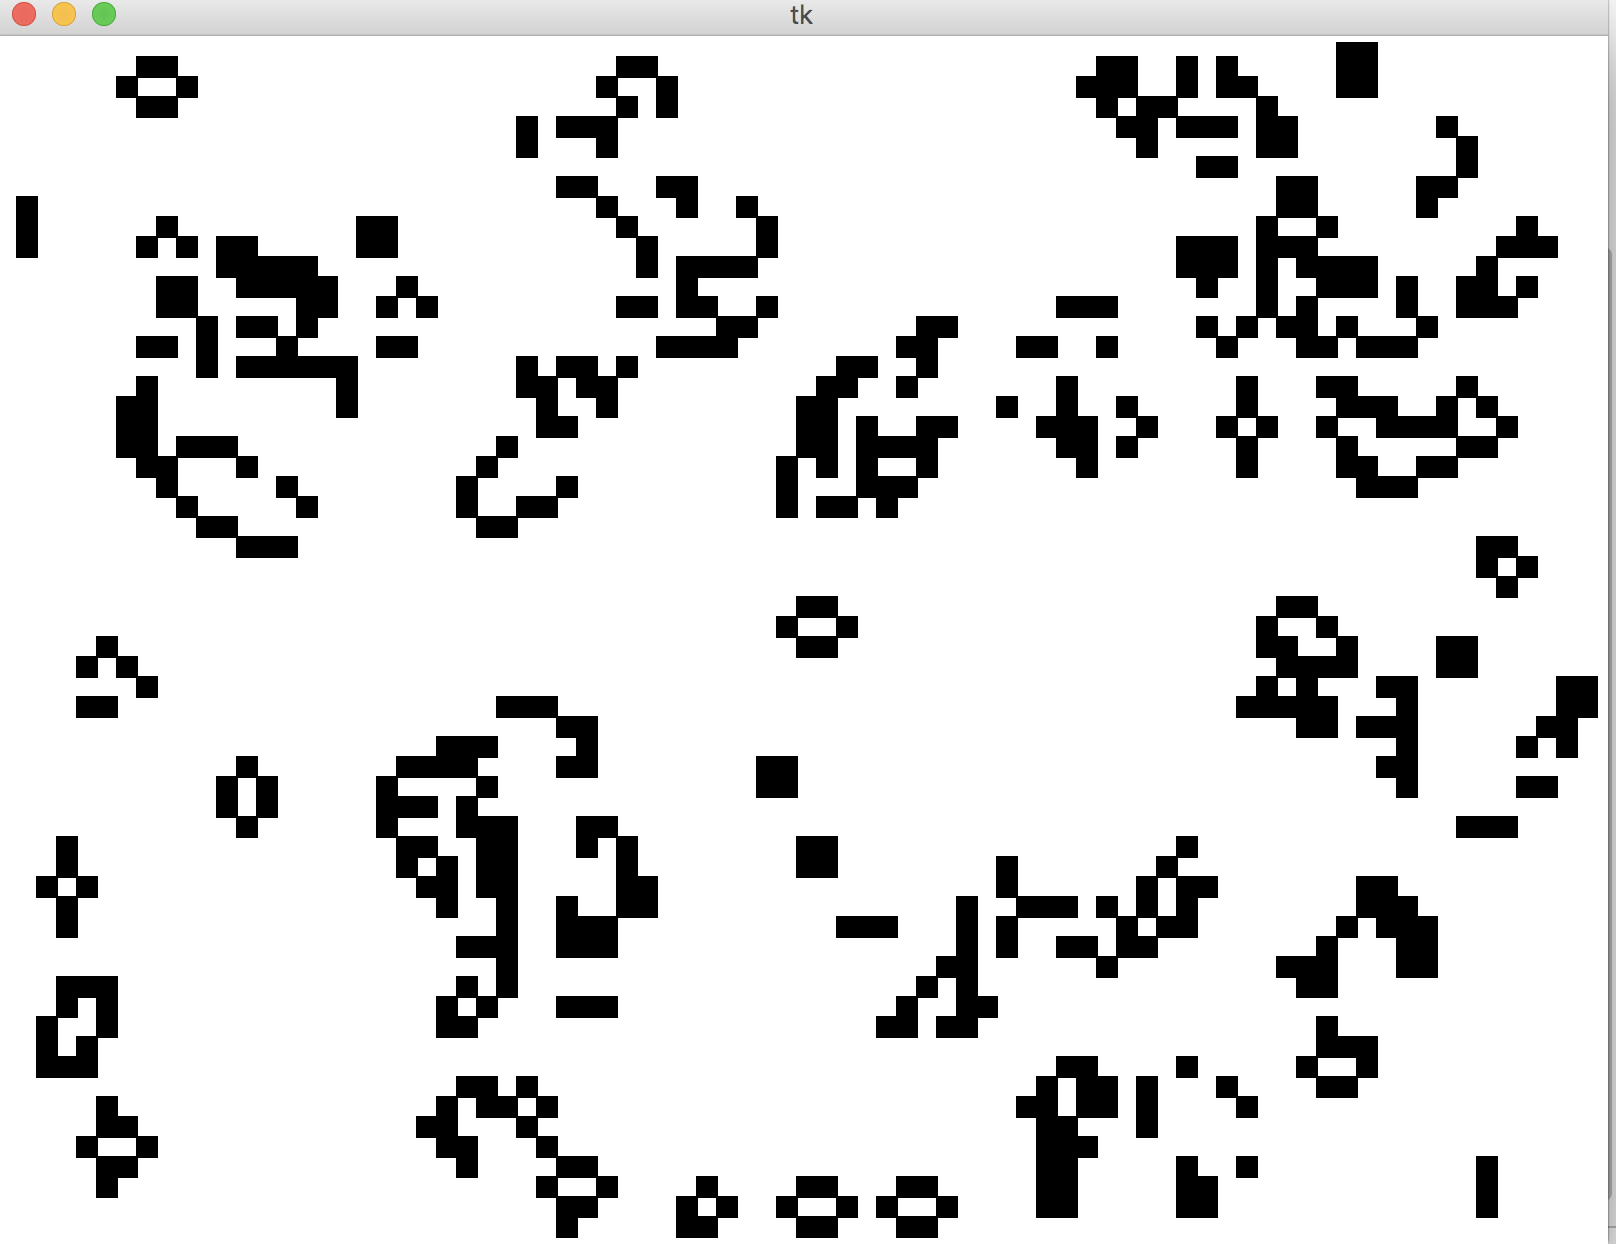
\includegraphics[height=0.4\textwidth]{img/i1}
    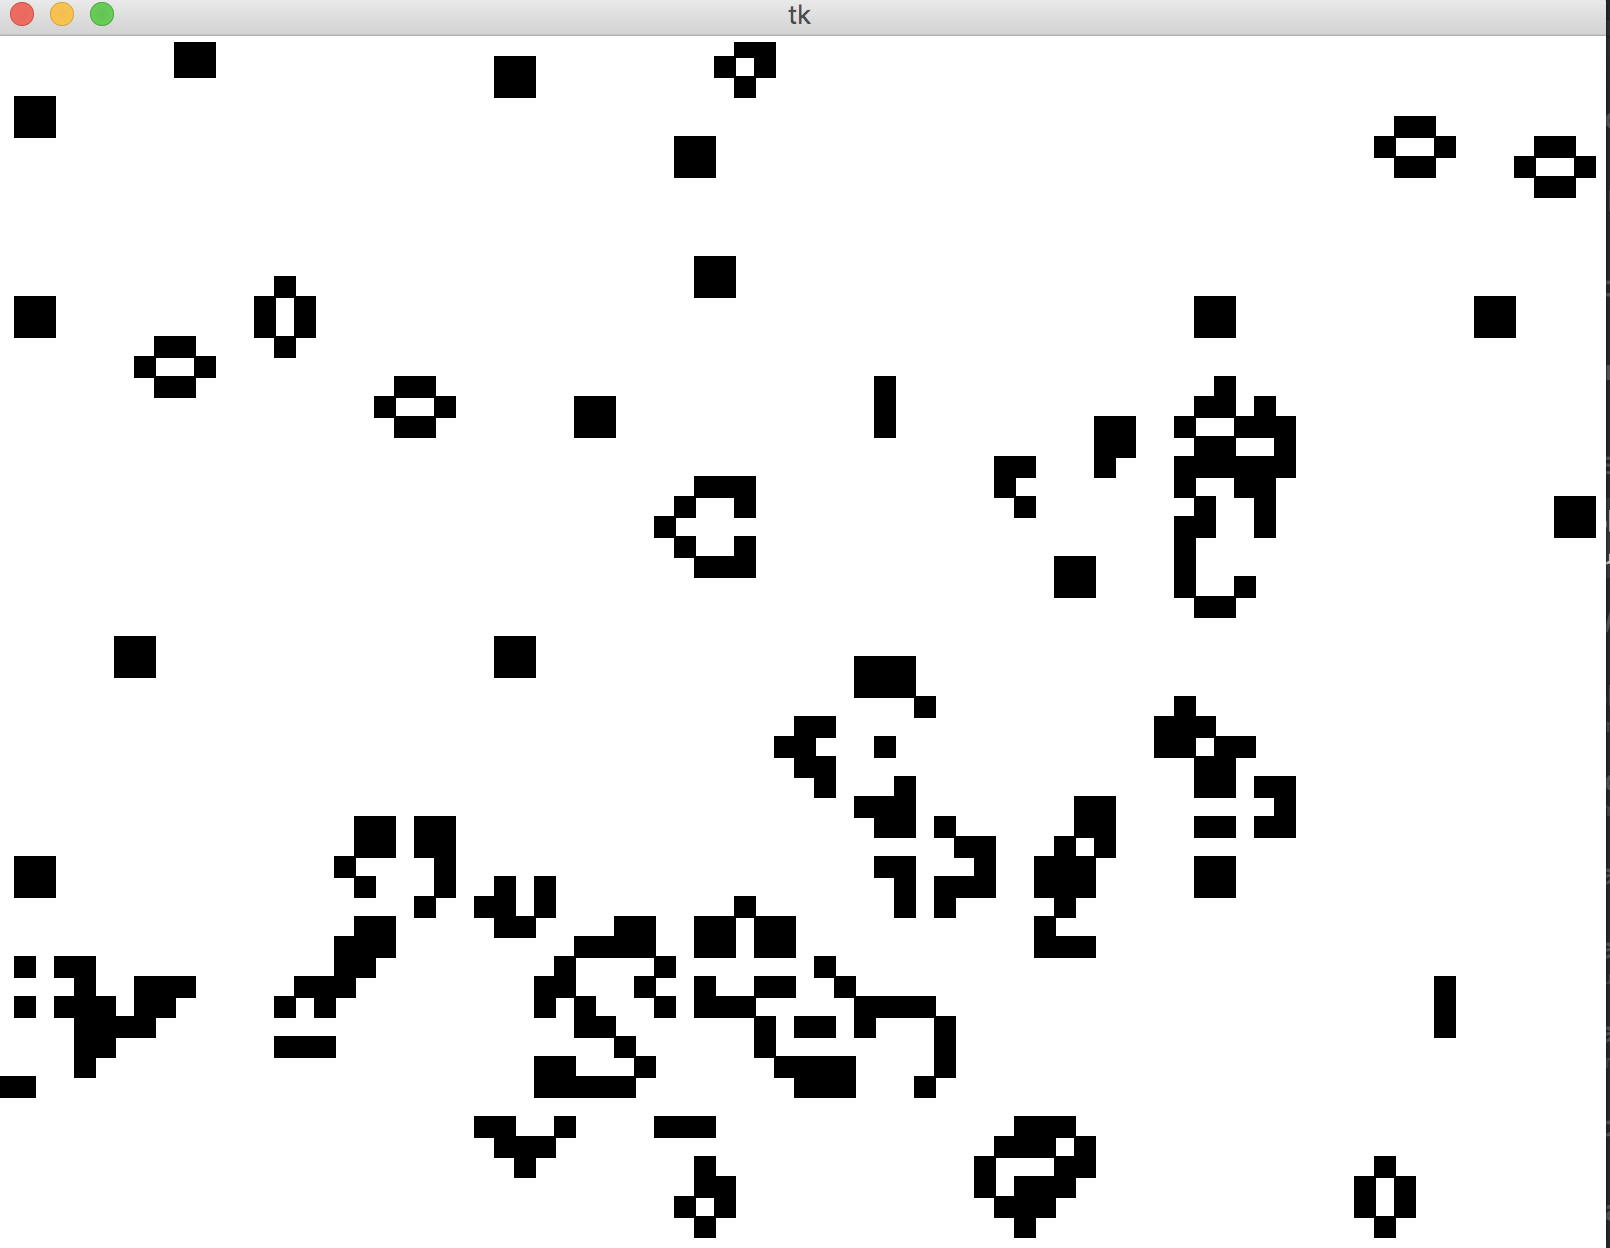
\includegraphics[height=0.4\textwidth]{img/i2}
    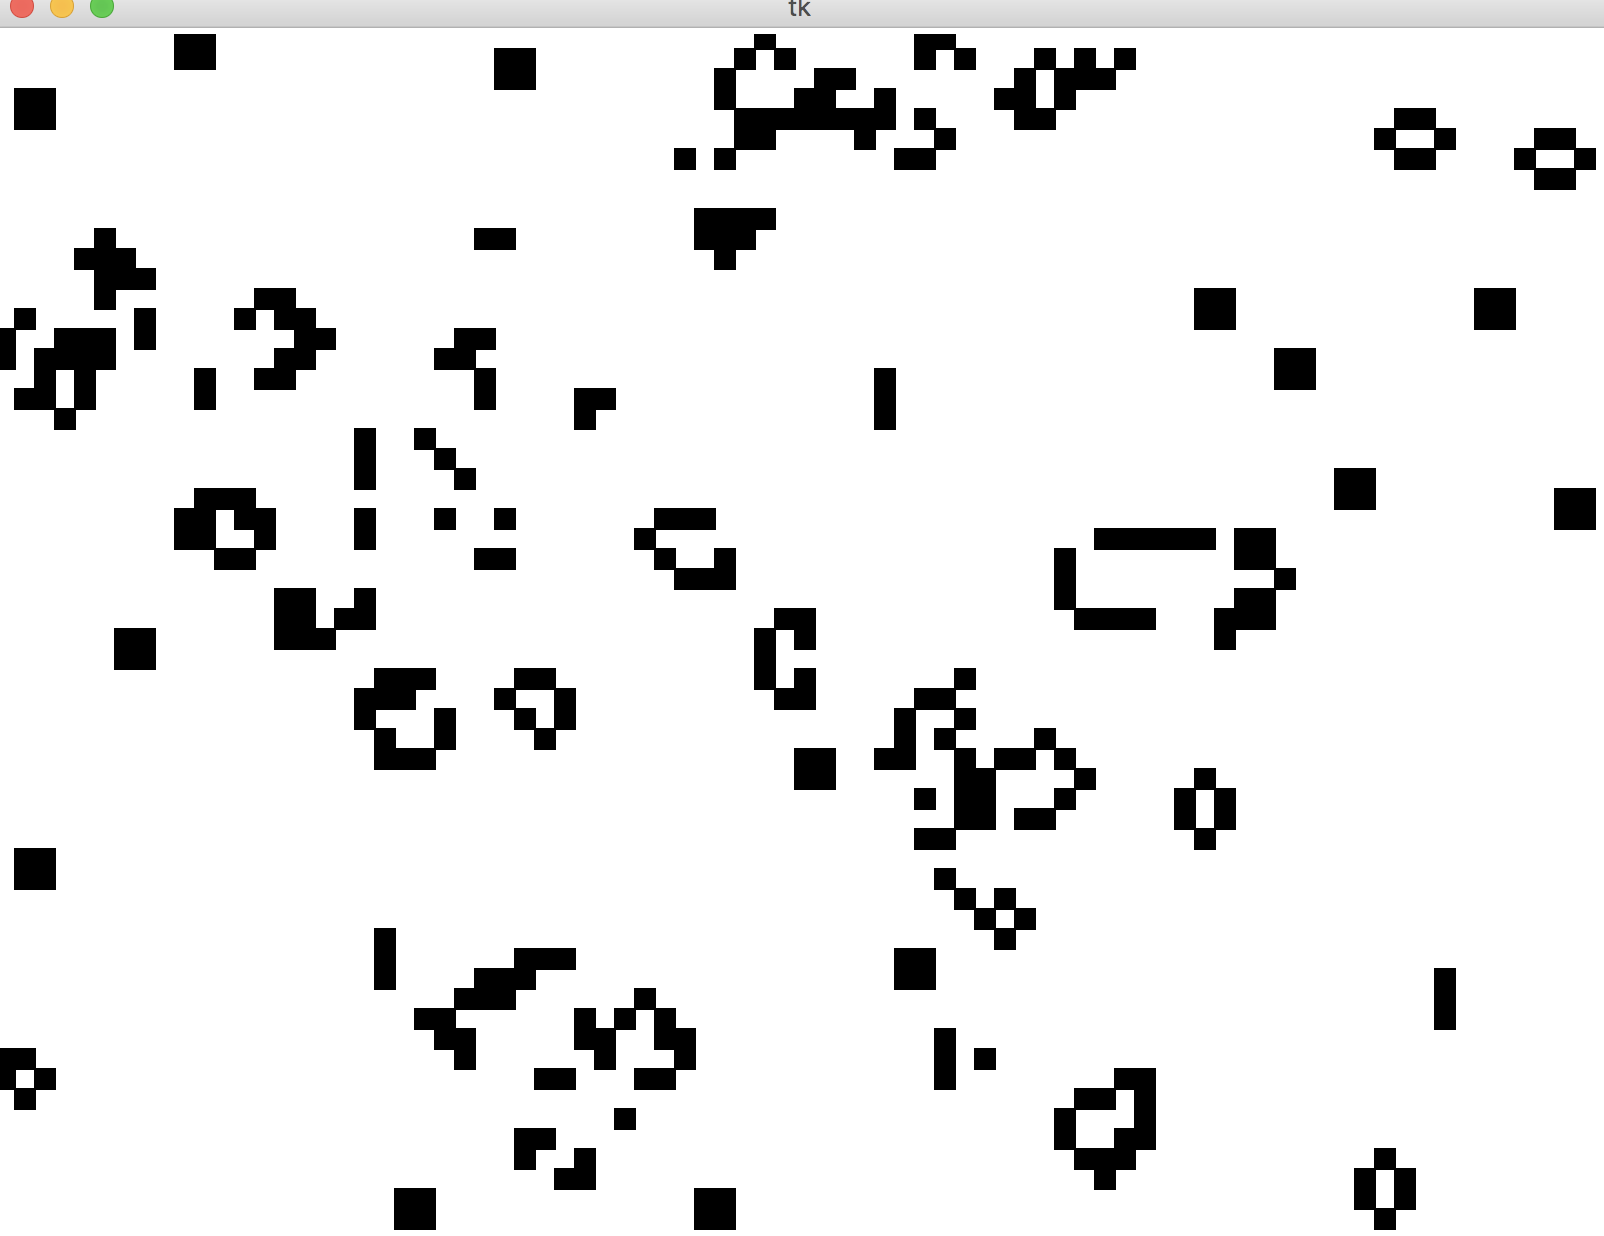
\includegraphics[height=0.4\textwidth]{img/i3}
    \caption{Exemples de générations du game of life}
    \label{fig:ending_examples}
\end{figure}
\]
\end{document}